\documentclass[UROP.tex]{subfiles}
\begin{document}

\bigskip
\section{\Large Methods}
\subsection{Antenna Design}

	To design the phased array system, we will begin by drafting a "bowtie" dipole antenna, which is a common and understood antenna type.  After this, we will arrange 16 antennas into two stacked rings of eight each.  We will be using this design at the behest of one of our mentors at the First RF Corporation, an antenna systems design company.  To verify our design, we will use FEKO and HFSS which are two antenna simulation software tools. \\

	The antenna will consist of 16 elements, arranged in two separate 8 element rings, one above the other.  Each element is a "bowtie" dipole, oriented in the vertical position to provide a vertically polarized field.  The UAS is equipped with an ordinary dipole, also oriented in the vertical position so it can receive these fields.  \\
	
	\begin{figure}[H]
		\centering
		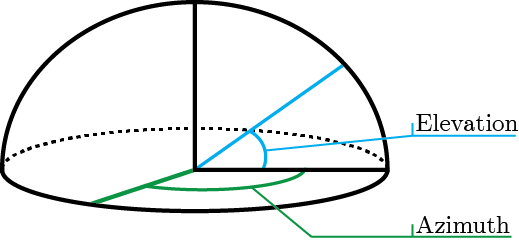
\includegraphics[]{elevation_azimuth.png}
		\caption{ Depiction of Azimuth and Elevation \label{fig:elevation_azimuth}}
	\end{figure}

	We are using this configuration because it should allow for the most signal coverage within the UAS airspace.  The ring of antennas allows for the beam to be steered 360 degrees around the system in azimuth.  The stacked rings allows for the beam to be pointed up and down in elevation.  Azimuth and elevation can be seen in Fig.~\ref{fig:elevation_azimuth}.  \\
	
	The UAS should be allowed to fly at distances up to 20 miles away while receiving data signals from the base station.  However, it will only fly at heights up to 200 meters so low elevation control is needed.  These two criterion are satisfied by the azimuth and elevation control of the beam.  \\

	%A dual ring phased array design will allow for more control in elevation.  The second, higher ring also creates more power at lower elevations.  The drone can and will fly at distances 20 miles away, at heights of 200 meters, so low elevation power is needed.  The design will also have 360$^{\circ}$ of azimuth.  A depiction of elevation compared to azimuth can be seen in Fig.~\ref{fig:elevation_azimuth}. \\
	
\subsection{Phased Array Control System}

	Controlling the direction of the beam requires changing the phase and amplitude of each antenna array element.  The elements will be initially fed with the same signal, but then attenuated and/or phase shifted to steer the beam towards the drone.  This method is used by other phased array system designers, including our mentors at the First RF Corporation.  \\
	
	The control system will be managed by an STM processor.  This processor will be in charge of outputting correct phases and amplitudes to the phased array elements.  Calculations to determine the correct phase and amplitude values to steer the beam require rigorous testing and analysis.  Formulas exist for ideal isotropic antenna elements to determine phase and amplitude values, however this new design requires more intensive research to create accurate formulas.  During antenna simulations, methods will be constructed to help provide guidance to the control system in order to steer the beam correctly. \\
	
\end{document}
